\documentclass[a4paper,12pt]{article}

\usepackage[UTF8]{ctex}
\usepackage{geometry}
\usepackage{graphicx}
\usepackage{float}
\usepackage{booktabs}
\usepackage{array}
\usepackage{caption}
\usepackage{subcaption}
\usepackage{xcolor}
\usepackage{hyperref}
\usepackage{fancyhdr}
\usepackage{titlesec}
\usepackage{enumitem}
\usepackage{tikz}
\usetikzlibrary{arrows.meta,positioning}

\geometry{left=2.0cm,right=2.0cm,top=2.2cm,bottom=2.2cm}
\hypersetup{hidelinks,pdfencoding=unicode}
\setlength{\parindent}{2em}
\setlength{\parskip}{0.35em}
\renewcommand{\arraystretch}{1.2}

\definecolor{theme}{RGB}{27,86,140}
\titleformat{\section}{\Large\bfseries\color{theme}}{\thesection}{0.8em}{}
\titleformat{\subsection}{\large\bfseries\color{theme}}{\thesubsection}{0.6em}{}

\pagestyle{fancy}
\fancyhf{}
\fancyhead[L]{计算机控制系统设计与实践}
\fancyhead[R]{作业3}
\fancyfoot[C]{\thepage}
\setlength{\headheight}{15pt}

\newcommand{\reporttitle}{
  \begin{center}
    {\zihao{2}\bfseries 作业3\par}
    \vspace{0.5em}
    {\large PLC 控制程序设计\par}
    \vspace{1em}
    \begin{tabular}{p{3cm}p{4.5cm}p{3cm}p{4.5cm}}
      \toprule
      姓名 & 陈卓 & 学号 & 3230104877 \\
      \bottomrule
    \end{tabular}
  \end{center}
}

\begin{document}

\reporttitle

\section{实验任务与资料说明}
本报告依据课程作业要求完成两部分内容：
\begin{enumerate}[leftmargin=2em]
  \item 第一问：依据给定程序与参考资料，对现有喷泉控制逻辑进行整理、说明与结果分析。
  \item 第二问：在相同平台上自主提出一个可实现的扩展控制方案，仅提交设计思路与梯形图，不要求完整仿真工程文件。
\end{enumerate}

题目原始示意图如图~\ref{fig:task-origin} 所示，喷头分为 A、B 两组，每组 6 个喷头。

\begin{figure}[H]
  \centering
  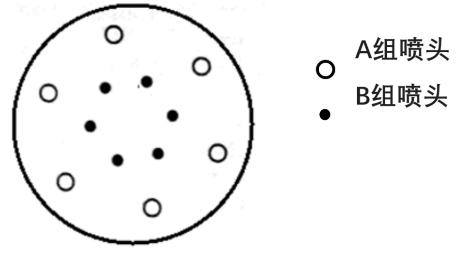
\includegraphics[width=0.72\linewidth]{assets/image1_image1.png}
  \caption{题目中的喷头分组示意}
  \label{fig:task-origin}
\end{figure}

\section{第一问：参考程序分析与结果}
\subsection{控制要求重述}
根据题意，系统在按下启动按钮后应按如下顺序循环运行：
\begin{enumerate}[leftmargin=2em]
  \item A 组喷头与水泵 P1 动作 6 s；
  \item B 组喷头与水泵 P2 动作 6 s；
  \item A、B 两组同时动作 6 s；
  \item 全部停止 3 s 后再次循环。
\end{enumerate}
按下停止按钮后应立即停止全部喷头与水泵。

\subsection{I/O 分配}
参考程序采用的地址映射见图~\ref{fig:io-map}。

\begin{figure}[H]
  \centering
  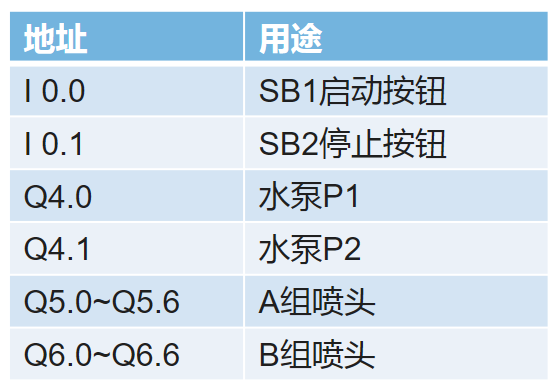
\includegraphics[width=0.65\linewidth]{assets/image2_image2.png}
  \caption{第一问 I/O 地址分配}
  \label{fig:io-map}
\end{figure}

\subsection{程序结构说明}
参考解将逻辑分为 3 个程序段：工作状态自锁、定时链、输出控制。

\textbf{(1) 工作状态自锁}\\
通过启动/停止按钮构成典型起保停回路，内部位 \texttt{M0.0} 表示系统工作状态。程序截图见图~\ref{fig:nw1}。

\begin{figure}[H]
  \centering
  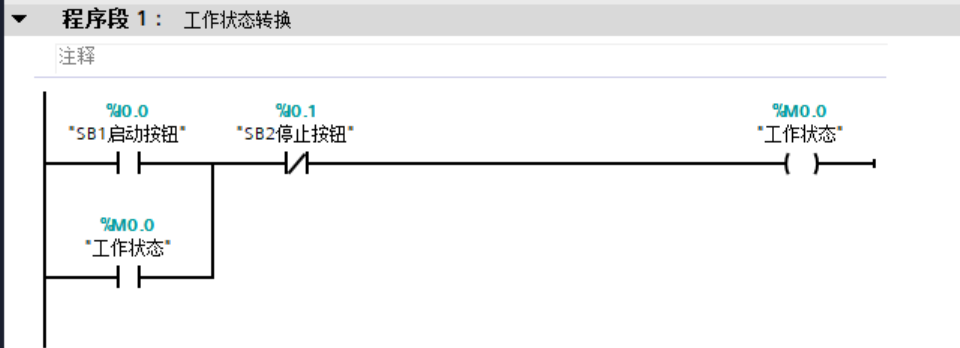
\includegraphics[width=0.82\linewidth]{assets/image3_image3.png}
  \caption{程序段 1：工作状态控制}
  \label{fig:nw1}
\end{figure}

\textbf{(2) 定时链}\\
使用 \texttt{Timer1\textasciitilde Timer4} 串联形成周期节拍：6 s + 6 s + 6 s + 3 s。对应逻辑如图~\ref{fig:nw2-overview}、图~\ref{fig:nw2-compact}。

\begin{figure}[H]
  \centering
  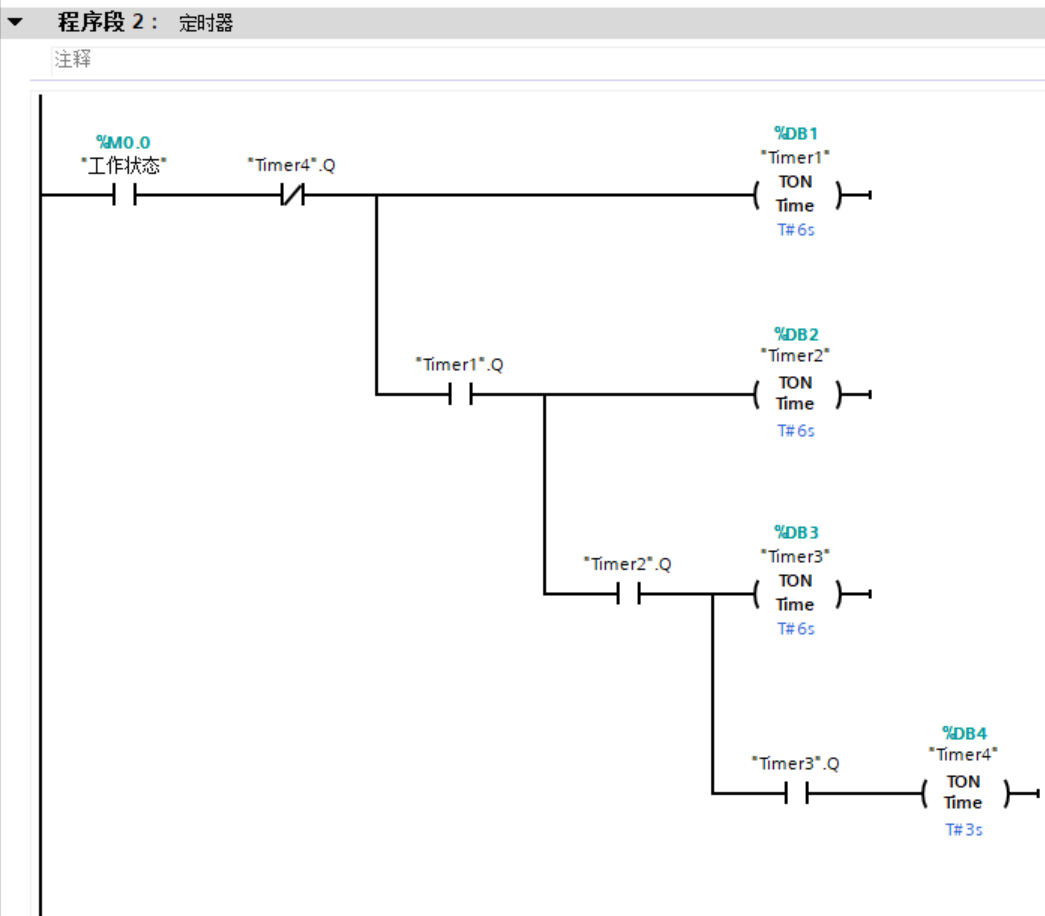
\includegraphics[width=\linewidth]{assets/image4_image4.png}
  \caption{程序段 2：定时器分支结构}
  \label{fig:nw2-overview}
\end{figure}

\begin{figure}[H]
  \centering
  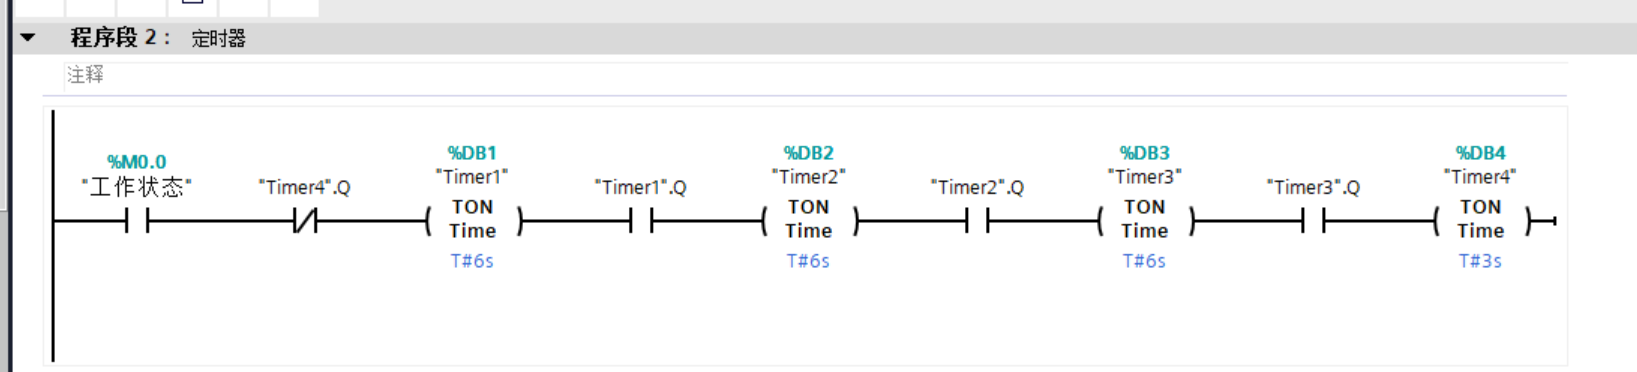
\includegraphics[width=\linewidth]{assets/image5_image5.png}
  \caption{程序段 2：定时器串联紧凑写法}
  \label{fig:nw2-compact}
\end{figure}

\textbf{(3) 输出控制}\\
依据各定时器 \texttt{Q} 位组合，分别驱动 A 组、B 组喷头及对应水泵，程序见图~\ref{fig:nw3}。

\begin{figure}[H]
  \centering
  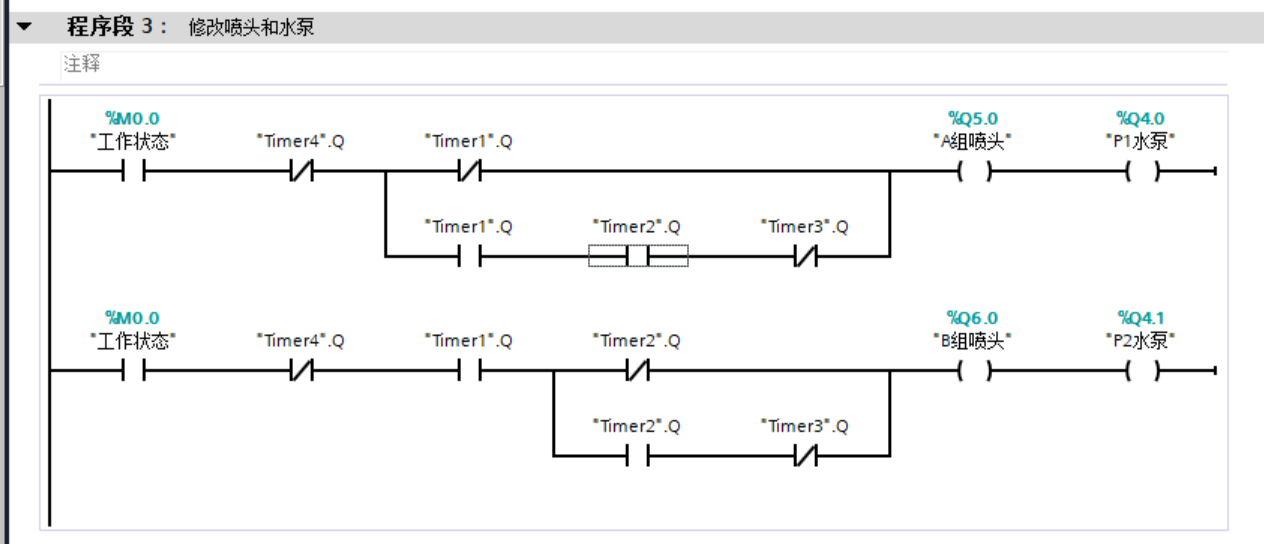
\includegraphics[width=\linewidth]{assets/image6_image6.png}
  \caption{程序段 3：喷头与水泵输出逻辑}
  \label{fig:nw3}
\end{figure}

\subsection{仿真轨迹与结果分析}
仿真波形见图~\ref{fig:trace}，可观察到：
\begin{itemize}[leftmargin=2em]
  \item \texttt{P1} 与 \texttt{P2} 在 6 s、6 s、6 s、3 s 周期中按要求交替/同时动作；
  \item 工作状态位保持有效时周期重复；
  \item 在停止条件触发后，输出立即复位，满足题目要求。
\end{itemize}

\begin{figure}[H]
  \centering
  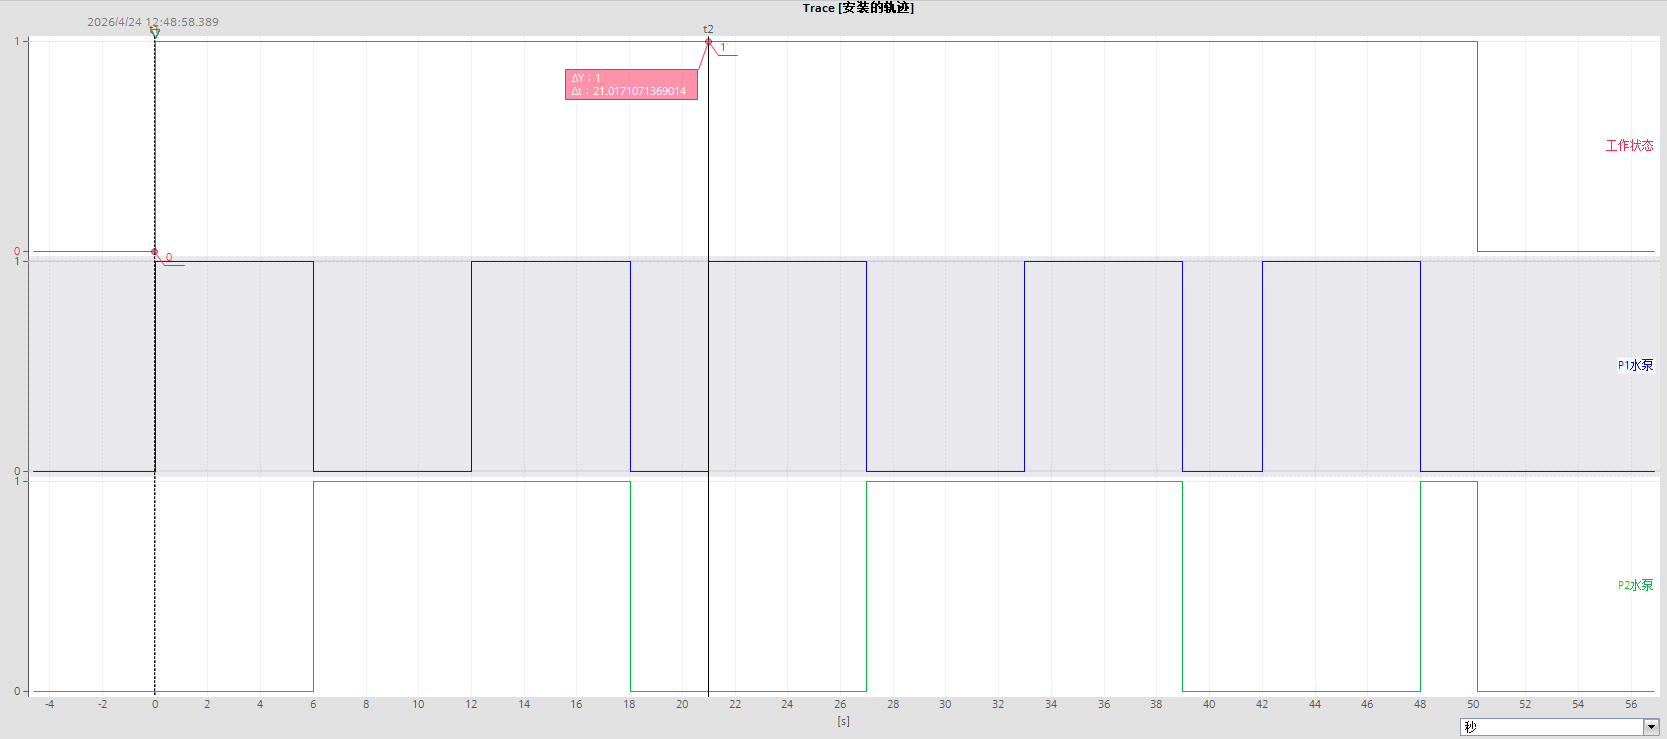
\includegraphics[width=\linewidth]{assets/image7_image7.png}
  \caption{参考程序 Trace 波形}
  \label{fig:trace}
\end{figure}

\subsection{思考题：将水泵改为开度可调（Real）}
参考资料给出的做法是把 \texttt{P1}、\texttt{P2} 由 \texttt{Bool} 扩展为 \texttt{Real}，增加 \texttt{水泵开度} 变量，通过 \texttt{MOVE} 指令在“应开启”时写入开度值、在“应关闭”时写入 \texttt{0.0}。变量示例与逻辑示例如图~\ref{fig:var-real}、图~\ref{fig:move-real}。

\begin{figure}[H]
  \centering
  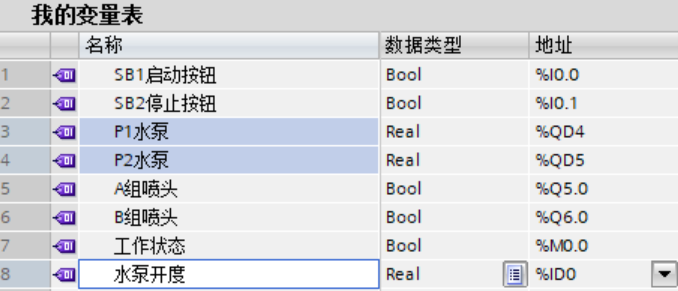
\includegraphics[width=0.78\linewidth]{assets/image8_image8.png}
  \caption{变量表扩展示例（含 Real 开度）}
  \label{fig:var-real}
\end{figure}

\begin{figure}[H]
  \centering
  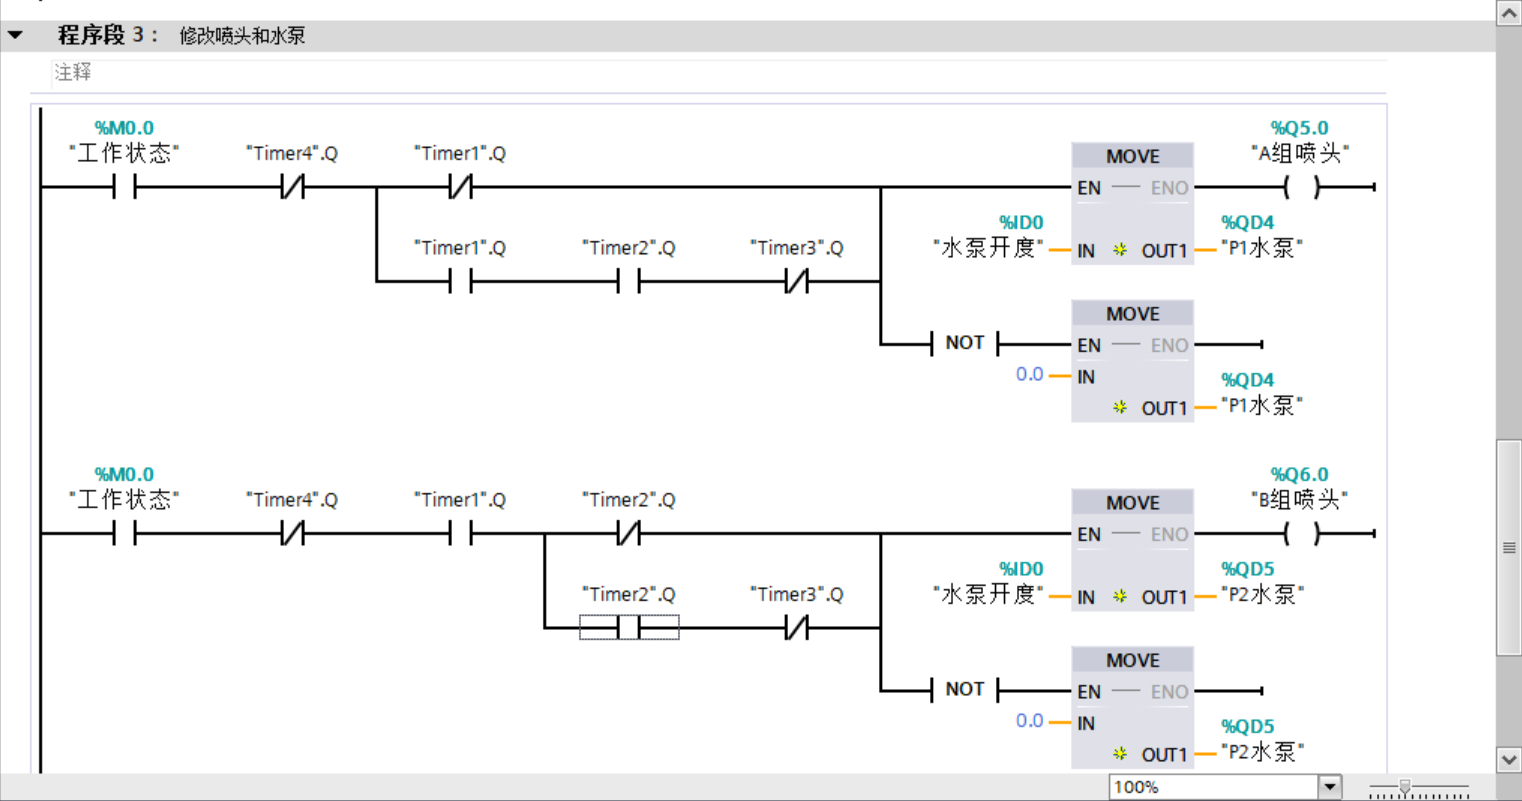
\includegraphics[width=\linewidth]{assets/image9_image9.png}
  \caption{Real 开度输出的 MOVE 实现示例}
  \label{fig:move-real}
\end{figure}

\section{第二问：自主设计方案（含梯形图）}
\subsection{设计目标}
在第一问基础上，提出“\textbf{双模式喷泉控制}”方案：
\begin{itemize}[leftmargin=2em]
  \item \textbf{自动模式}：沿用原 6+6+6+3 s 节拍；
  \item \textbf{手动模式}：操作员可单独点动 A 组或 B 组喷头；
  \item \textbf{安全联锁}：液位低或急停触发时，所有输出强制关闭；
  \item \textbf{工程化}：保持状态位、模式位、报警位分层，便于后续扩展到 HMI。
\end{itemize}

\subsection{建议 I/O 与内部变量}
\begin{table}[H]
  \centering
  \caption{第二问建议变量分配}
  \begin{tabular}{p{3cm}p{3cm}p{7.2cm}}
    \toprule
    变量 & 类型/地址 & 说明 \\
    \midrule
    SB1\_Start & I0.0 (Bool) & 启动按钮 \\
    SB2\_Stop & I0.1 (Bool) & 停止按钮 \\
    SA\_Mode & I0.2 (Bool) & 模式选择：0 自动，1 手动 \\
    SB\_A\_Jog & I0.3 (Bool) & 手动 A 组点动 \\
    SB\_B\_Jog & I0.4 (Bool) & 手动 B 组点动 \\
    LS\_LowLevel & I0.5 (Bool) & 低液位开关（1 表示液位低） \\
    M\_Run & M0.0 (Bool) & 系统运行状态 \\
    M\_Auto & M0.1 (Bool) & 自动模式有效 \\
    Q\_P1 / Q\_P2 & Q4.0 / Q4.1 & 两组水泵输出 \\
    Q\_A / Q\_B & Q5.0 / Q6.0 & 两组喷头主控输出 \\
    \bottomrule
  \end{tabular}
\end{table}

\subsection{控制流程}
\begin{enumerate}[leftmargin=2em]
  \item 通过起保停回路生成 \texttt{M\_Run}；
  \item 当 \texttt{LS\_LowLevel=1} 或停止按钮按下，\texttt{M\_Run} 立即断开；
  \item 自动模式下，按 \texttt{Timer1\textasciitilde Timer4} 产生节拍并驱动输出；
  \item 手动模式下，\texttt{SB\_A\_Jog}/\texttt{SB\_B\_Jog} 直接驱动对应组，且互不影响；
  \item 输出层统一经过 \texttt{M\_Run} 与安全联锁门控，保证故障时全停。
\end{enumerate}

\subsection{梯形图设计（方案图）}
图~\ref{fig:q2-ladder} 给出第二问核心梯形图（设计方案级）。其核心思想是“\textbf{模式选择在中间层，安全联锁在输出层前统一收口}”，便于调试和扩展。

\begin{figure}[H]
  \centering
  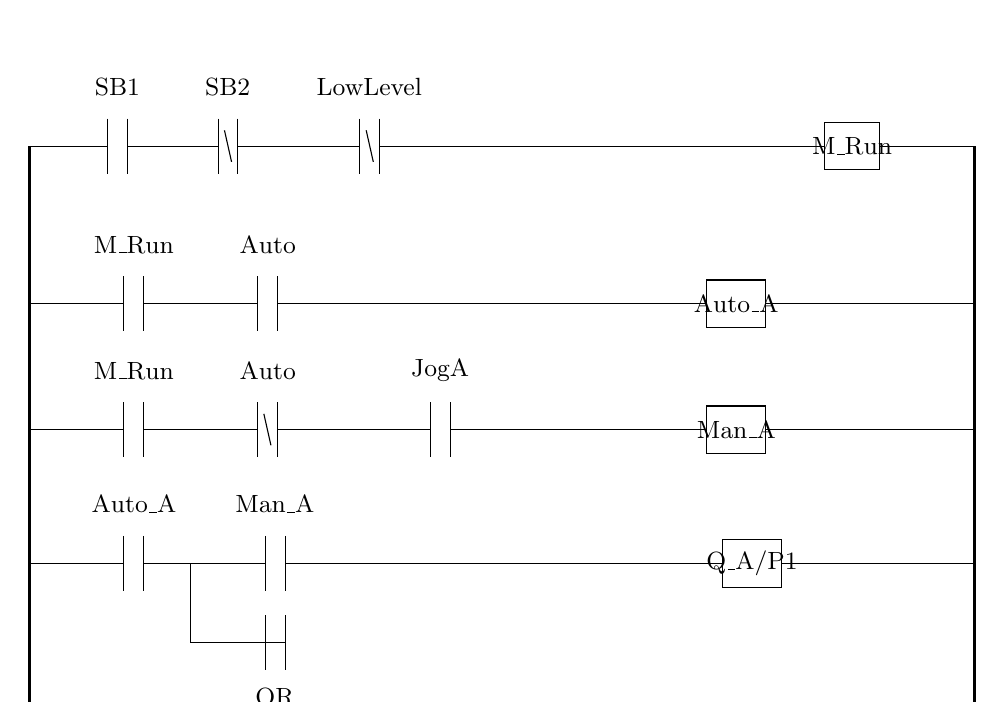
\begin{tikzpicture}[x=1cm,y=1cm,>=Latex]
    % rails
    \draw[line width=1.1pt] (0,0) -- (0,-7.2);
    \draw[line width=1.1pt] (12,0) -- (12,-7.2);

    % rung 1
    \draw (0,0) -- (1.0,0);
    \draw (1.0,0.35) -- (1.0,-0.35); \draw (1.25,0.35) -- (1.25,-0.35);
    \node[font=\small] at (1.12,0.75) {SB1};
    \draw (1.25,0) -- (2.4,0);
    \draw (2.4,0.35) -- (2.4,-0.35); \draw (2.65,0.35) -- (2.65,-0.35);
    \draw (2.48,0.2) -- (2.57,-0.2);
    \node[font=\small] at (2.52,0.75) {SB2};
    \draw (2.65,0) -- (4.2,0);
    \draw (4.2,0.35) -- (4.2,-0.35); \draw (4.45,0.35) -- (4.45,-0.35);
    \draw (4.28,0.2) -- (4.37,-0.2);
    \node[font=\small] at (4.32,0.75) {LowLevel};
    \draw (4.45,0) -- (10.1,0);
    \draw (10.1,0.3) -- (10.8,0.3) -- (10.8,-0.3) -- (10.1,-0.3) -- cycle;
    \node[font=\small] at (10.45,0) {M\_Run};
    \draw (10.8,0) -- (12,0);

    % rung 2
    \draw (0,-2) -- (1.2,-2);
    \draw (1.2,-1.65) -- (1.2,-2.35); \draw (1.45,-1.65) -- (1.45,-2.35);
    \node[font=\small] at (1.33,-1.25) {M\_Run};
    \draw (1.45,-2) -- (2.9,-2);
    \draw (2.9,-1.65) -- (2.9,-2.35); \draw (3.15,-1.65) -- (3.15,-2.35);
    \node[font=\small] at (3.03,-1.25) {Auto};
    \draw (3.15,-2) -- (8.6,-2);
    \draw (8.6,-1.7) -- (9.35,-1.7) -- (9.35,-2.3) -- (8.6,-2.3) -- cycle;
    \node[font=\small] at (8.98,-2) {Auto\_A};
    \draw (9.35,-2) -- (12,-2);

    % rung 3
    \draw (0,-3.6) -- (1.2,-3.6);
    \draw (1.2,-3.25) -- (1.2,-3.95); \draw (1.45,-3.25) -- (1.45,-3.95);
    \node[font=\small] at (1.33,-2.85) {M\_Run};
    \draw (1.45,-3.6) -- (2.9,-3.6);
    \draw (2.9,-3.25) -- (2.9,-3.95); \draw (3.15,-3.25) -- (3.15,-3.95);
    \draw (2.98,-3.4) -- (3.07,-3.8);
    \node[font=\small] at (3.03,-2.85) {Auto};
    \draw (3.15,-3.6) -- (5.1,-3.6);
    \draw (5.1,-3.25) -- (5.1,-3.95); \draw (5.35,-3.25) -- (5.35,-3.95);
    \node[font=\small] at (5.22,-2.85) {JogA};
    \draw (5.35,-3.6) -- (8.6,-3.6);
    \draw (8.6,-3.3) -- (9.35,-3.3) -- (9.35,-3.9) -- (8.6,-3.9) -- cycle;
    \node[font=\small] at (8.98,-3.6) {Man\_A};
    \draw (9.35,-3.6) -- (12,-3.6);

    % rung 4
    \draw (0,-5.3) -- (1.2,-5.3);
    \draw (1.2,-4.95) -- (1.2,-5.65); \draw (1.45,-4.95) -- (1.45,-5.65);
    \node[font=\small] at (1.33,-4.55) {Auto\_A};
    \draw (1.45,-5.3) -- (3.0,-5.3);
    \draw (3.0,-4.95) -- (3.0,-5.65); \draw (3.25,-4.95) -- (3.25,-5.65);
    \node[font=\small] at (3.12,-4.55) {Man\_A};
    \draw (2.05,-5.3) -- (2.05,-6.3) -- (3.25,-6.3);
    \draw (3.0,-6.65) -- (3.0,-5.95); \draw (3.25,-6.65) -- (3.25,-5.95);
    \node[font=\small] at (3.12,-7.0) {OR};
    \draw (3.25,-5.3) -- (8.8,-5.3);
    \draw (8.8,-5.0) -- (9.55,-5.0) -- (9.55,-5.6) -- (8.8,-5.6) -- cycle;
    \node[font=\small] at (9.18,-5.3) {Q\_A/P1};
    \draw (9.55,-5.3) -- (12,-5.3);
  \end{tikzpicture}
  \caption{第二问梯形图（自动/手动/联锁的核心结构）}
  \label{fig:q2-ladder}
\end{figure}

\subsection{方案特点与可实施性}
\begin{itemize}[leftmargin=2em]
  \item 在保留原题节拍控制逻辑的前提下，新增模式选择与安全联锁，改动量小；
  \item 梯形图结构清晰，可直接映射到 TIA Portal 的网络化实现；
  \item 便于后续继续扩展为“开度曲线控制”“故障报警记录”“HMI 参数化”。
\end{itemize}

\section{补充：晶体管共射放大电路原理图与实验结果}
\subsection{电路原理图提取}
从《晶体管共射放大电路》文档中提取的主电路如图~\ref{fig:ce-main-circuit}。该电路为典型分压偏置共射极放大器：输入经耦合电容 \(C_b\) 加到基极，集电极电阻 \(R_c\) 提供电压放大，发射极电阻 \(R_e\) 与旁路电容 \(C_e\) 决定交流增益与稳定性，输出经耦合电容 \(C_c\) 加到负载 \(R_L\)。

\begin{figure}[H]
  \centering
  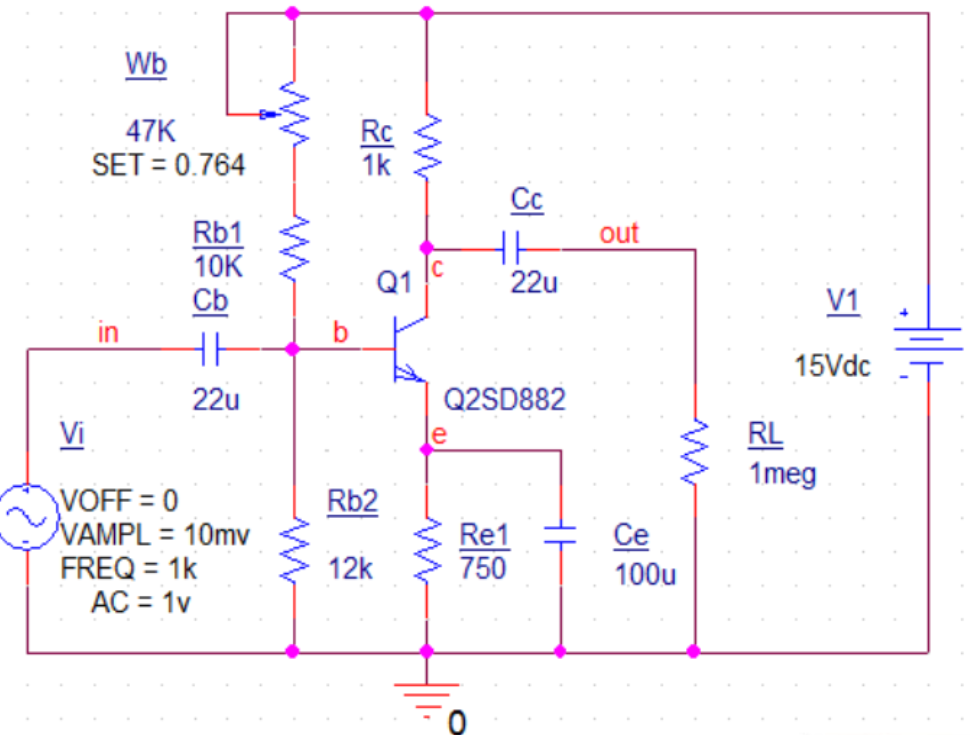
\includegraphics[width=0.78\linewidth]{assets/transistor/image4.png}
  \caption{晶体管共射放大电路原理图（由文档提取）}
  \label{fig:ce-main-circuit}
\end{figure}

\subsection{实验结果与数据整理}
根据文档中的示波器截图（见图~\ref{fig:ce-wave-a} 与图~\ref{fig:ce-wave-b}），读取到一组代表性结果。由于原始截图存在透视和亮度影响，数值按屏幕读数近似整理，保留 3 位有效数字用于报告展示。

\begin{table}[H]
  \centering
  \caption{共射放大实验截图读数整理}
  \begin{tabular}{p{2.1cm}p{3.2cm}p{3.2cm}p{4.8cm}}
    \toprule
    图号 & 输入有效值（约） & 输出有效值（约） & 说明 \\
    \midrule
    image9  & \(9.46\,\mathrm{mV}\) & \(1.55\,\mathrm{V}\) & 线性放大，输出与输入反相 \\
    image10 & \(10.5\,\mathrm{mV}\) & \(0.906\,\mathrm{V}\) & 小信号放大状态 \\
    image11 & \(14.0\,\mathrm{mV}\) & \(2.58\,\mathrm{V}\) & 增益较高，仍接近正弦 \\
    image14 & -- & \(2.86\,\mathrm{V}\) & 大信号测试截图 \\
    image15 & -- & \(1.93\,\mathrm{V}\) & 低频观测（\(T\approx 3.91\,\mathrm{ms}\)） \\
    image16 & -- & \(1.33\,\mathrm{V}\) & 高频/快速时基观测（\(f\approx 378.8\,\mathrm{Hz}\)） \\
    \bottomrule
  \end{tabular}
\end{table}

依据上述数据，可得到一组典型电压增益估算（以 image9 为例）：
\[
|A_v| \approx \frac{1.55}{9.46\times10^{-3}} \approx 1.64\times 10^2
\]
该数量级与共射极放大电路在旁路电容有效时的中频段高增益特性一致。

\begin{figure}[H]
  \centering
  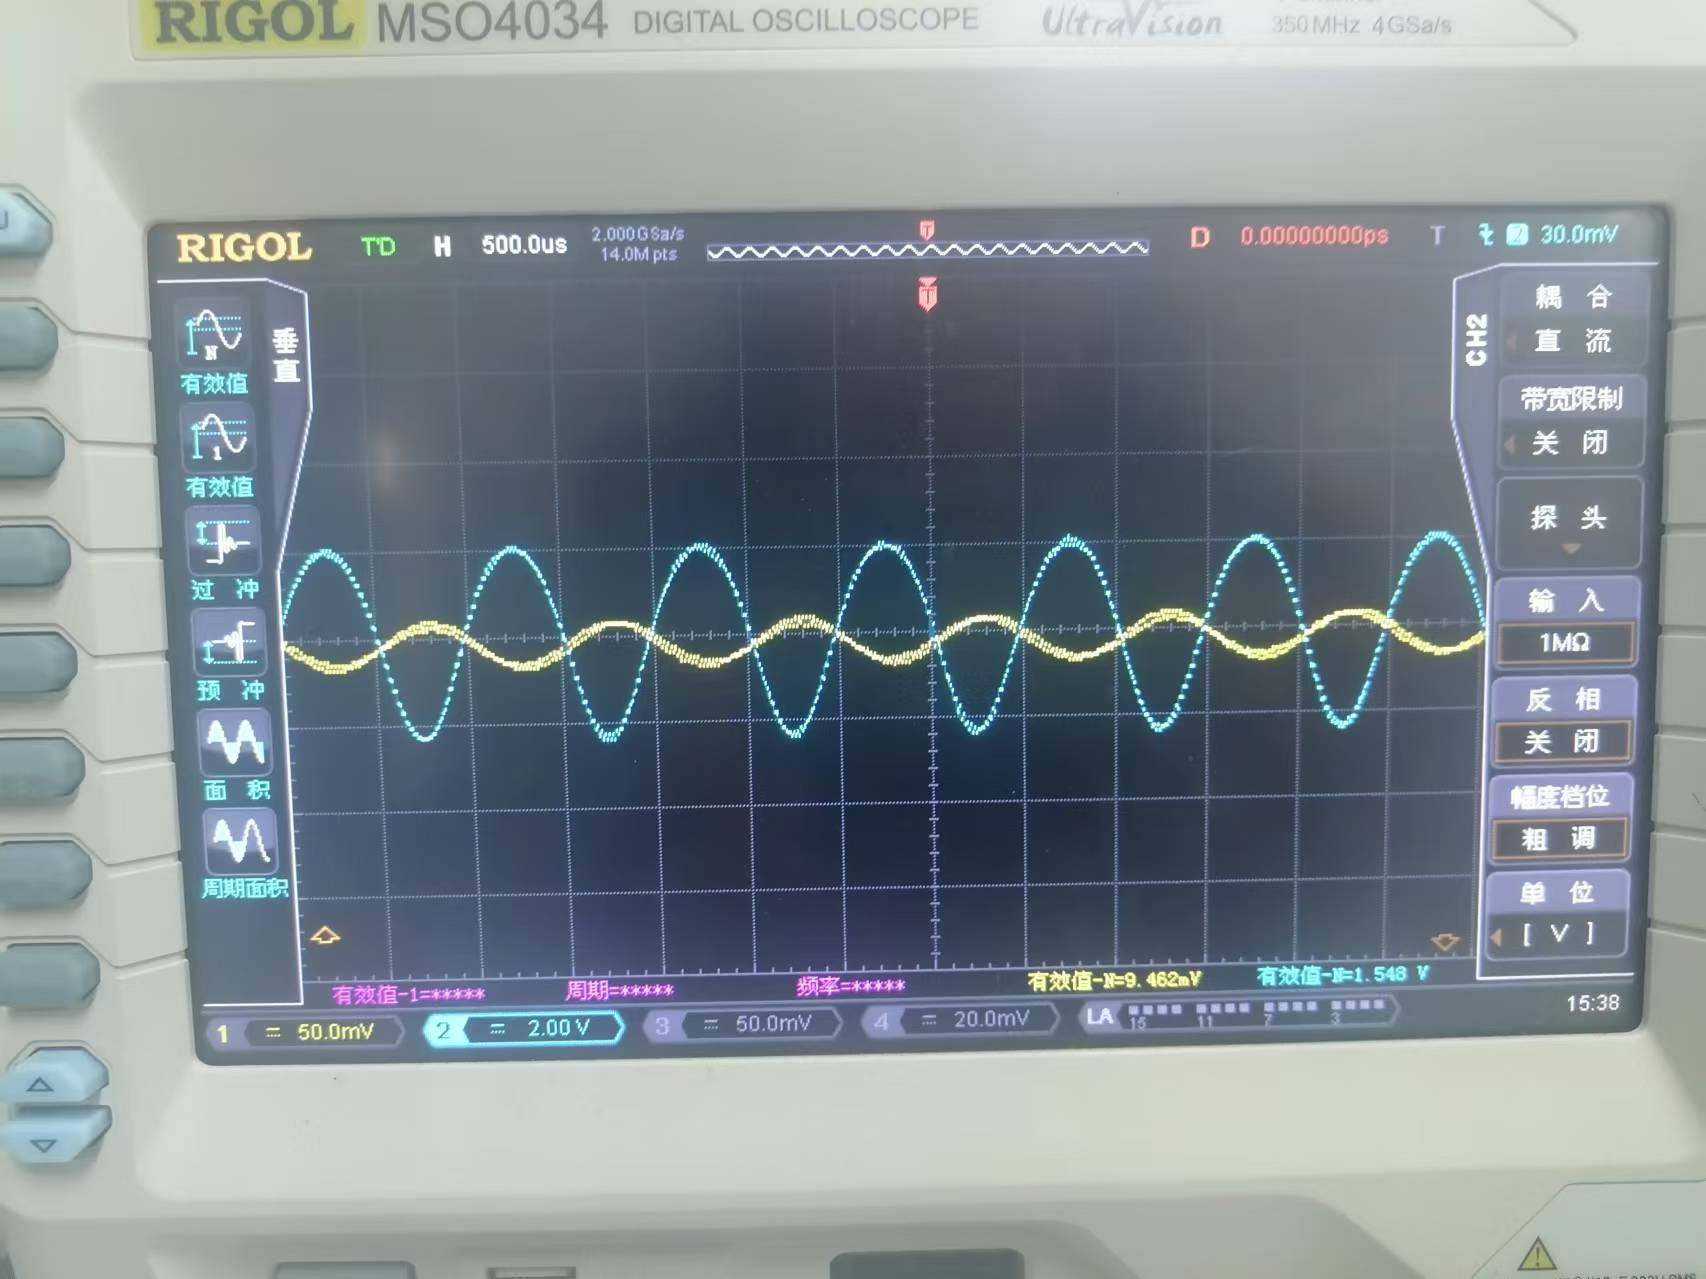
\includegraphics[width=0.49\linewidth]{assets/transistor/image9.jpeg}\hfill
  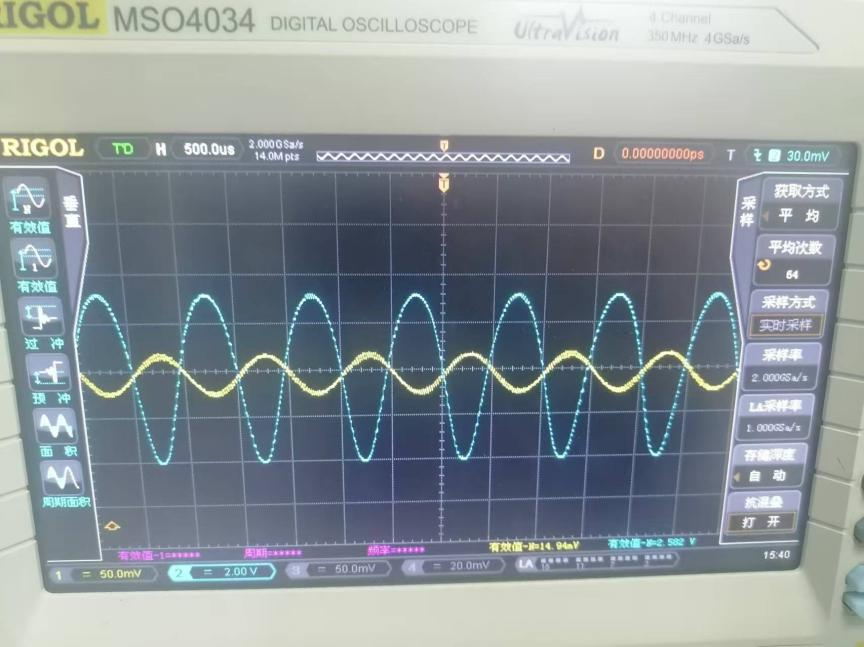
\includegraphics[width=0.49\linewidth]{assets/transistor/image11.jpeg}
  \caption{共射放大实验示波器截图（提取）}
  \label{fig:ce-wave-a}
\end{figure}

\begin{figure}[H]
  \centering
  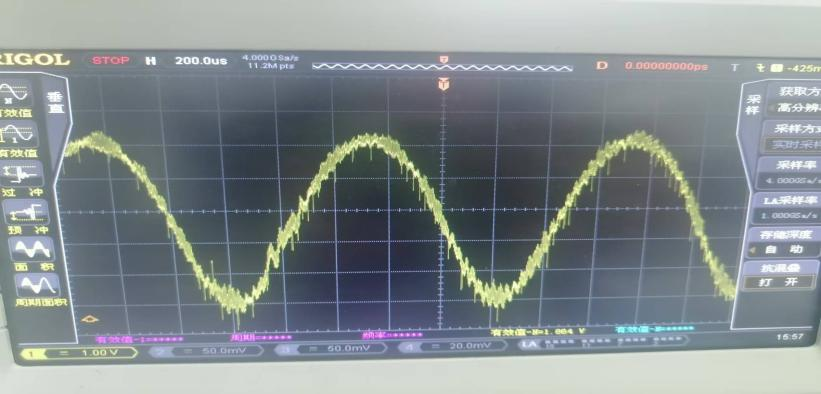
\includegraphics[width=0.49\linewidth]{assets/transistor/image14.jpeg}\hfill
  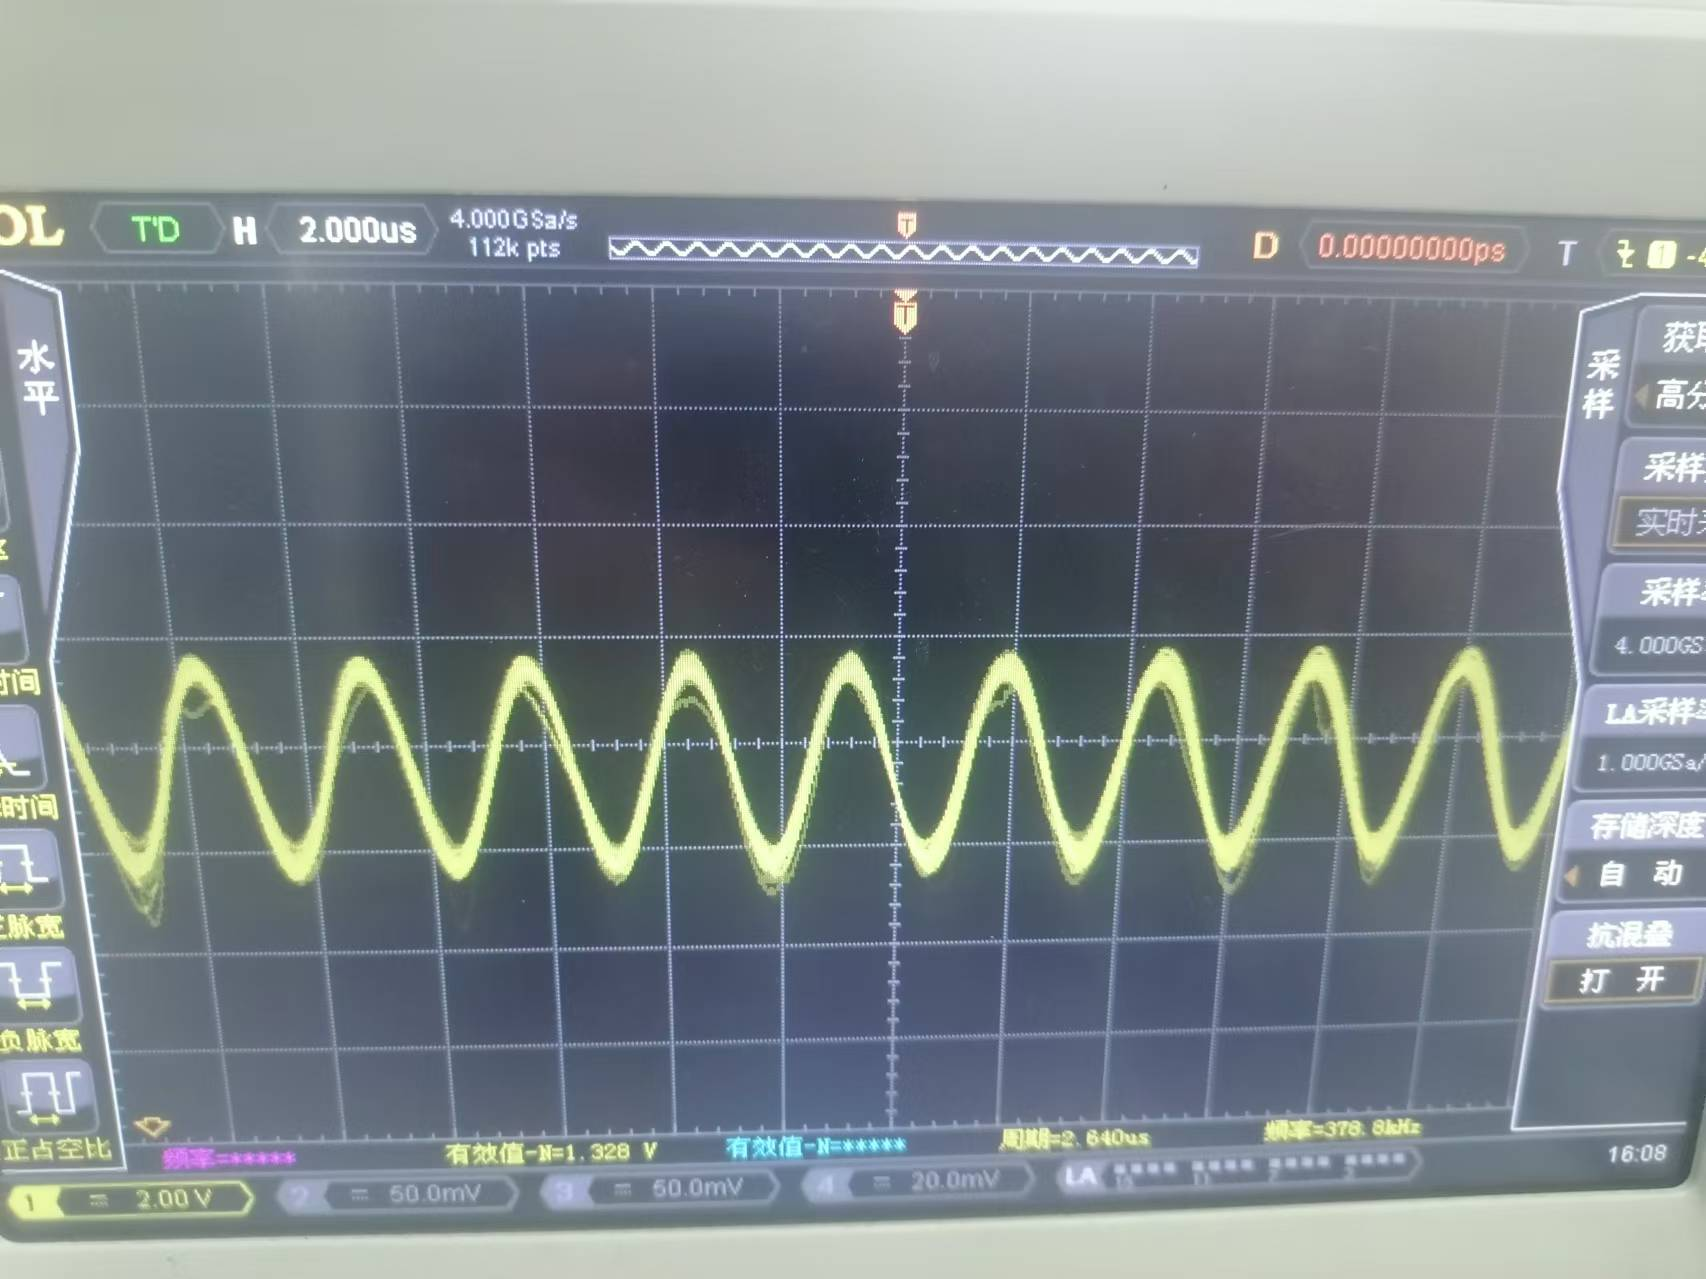
\includegraphics[width=0.49\linewidth]{assets/transistor/image16.jpeg}
  \caption{不同时基/幅值下的输出观测结果（提取）}
  \label{fig:ce-wave-b}
\end{figure}

\section{结论}
第一问已基于参考资料完成程序逻辑和波形结果分析，能够满足原题顺序与停止要求。第二问给出了可落地的扩展设计方案，并提供了可直接转化为 PLC 网络程序的梯形图结构，可作为后续工程实现基础。

\end{document}
